\chapter{Planificación}

\section{Gestión de recursos}
En este apartado describiré brevemente los recursos utilizados para llevar a cabo este proyecto tiendo en cuenta personal, hardware y software.

\subsection{Personal}
El único recurso humano que ha contribuido a la realización del proyecto soy yo mismo actuando como los diversos roles que llevan acabo el proceso de desarrollo de un proyecto de estas características.

\subsection{Hardware}
Respecto al hardware utilizado para este \acrshort{TFM} solo he requerido mi ordenador portátil personal, cuyas características se destacan en la siguiente tabla:

\begin{table} [h!]
\centering
\begin{tabular}{c c}
	\hline
	CPU & Intel \textregistered  Core \texttrademark  i7-4700MQ CPU @ 2.40GHz x 8\\
	RAM & 8 GB RAM DDR3\\
	Almacenamiento & HDD 750 GB (5400 RPM)\\
	\hline
\end{tabular}
	\caption{Especificaciones del equipo utilizado}
\end{table}

Esto ha bastado para el desarrollo, pero seria necesario conseguir un servidor en condiciones para llegar a poner en producción el sistema. Tampoco sería necesario nada muy potente ya que incluso en mi propio ordenador los tiempos empleados en la búsqueda son bastante aceptables.

\subsection{Software}
Se han empleado utilidades de software libre en la totalidad del proyecto. Aquí enumerare el principal software empleado y su función primordial, para una descripción más detalladas de las herramientas empleadas ver el capítulo \nameref{ch:herramientas}:

\begin{itemize}
	\item \textbf{Debian}: \acrfull{SO}.
	\item \textbf{Python}: Lenguaje de programación usado en las primeras fases del proyecto y en servidor \gls{backend} \glsrefentry{backend}.
	\item \textbf{JavaScript}: Lenguaje de programación interpretado en el que se ha escrito el \gls{frontend} \glsrefentry{frontend}.
	\item \textbf{Elasticsearch}: Servidor de búsqueda.
	\item \textbf{MongoDB}: Base de datos NoSQL.
	\item \textbf{React}:  \Gls{framework} para el desarrollo de interfaces de usuario.
	\item \textbf{Searchkit}: \Gls{framework} que incluye un conjunto de componentes React para la comunicación con Elasticsearch.
	\item \textbf{TeXstudio}: Entorno integrado de escritura en \LaTeX{} utilizado para generación de la documentación.
	\item \textbf{Docker}: Software de virtualización para basado en contenedores. Permite gestionar de forma simple la gestión y despliegue de una infraestructura software.
	\item \textbf{Visual Studio Code}: Editor de código creado por Microsoft utilizado para toda la programación del proyecto.
	
\end{itemize}

\section{Metodología}
\label{sc:metodologia}
Para desarrollar este proyecto se ha empleado una metodología ágil similar a \textit{\GLS{Scrum}} \glsrefentry{Scrum} algo más relajada. Es una modelo particular ya que yo mismo soy el desarrollador, el coordinador (rol del \textit{Scrum master}) y la persona encargada de definir las tareas y evaluar el cumplimiento de los mismas (el \textit{Product owner}).

Me he decantado por este modelo ya que permite más flexibilidad al enfrentarse a problemas en entornos desconocidos, como es este proyecto, y he tenido buena experiencia con él tanto en mi \acrshort{TFG} como durante mi vida laboral. Se basa en la descomposición del proyecto completo en pequeños subproyectos o \textit{sprints}, en los que define de manera acotada las tareas y objetivo del mismo. Permitiendo el refinamiento iterativo del producto final así como el aprovechamiento del conocimiento obtenido a lo largo de los sprint para mejorar los venideros, al contrario que otros modelos de desarrollo más clásicos que resultan más estáticos y rígidos.

Con el objetivo de almacenar y versionar todo el material producido en este proyecto he utilizado la plataforma \textit{GitHub} y el sistema de control de versiones \textit{git}.

Para seguir el progreso de cada uno de los \textit{sprints} del proyecto he utilizado los tableros que ofrece el propio \textit{GitHub projects} donde cada una de sus tareas o tarjetas corresponden con \textit{issues} como se puede ver en la siguiente imagen. 

\begin{figure}[h]
	
	\centering
	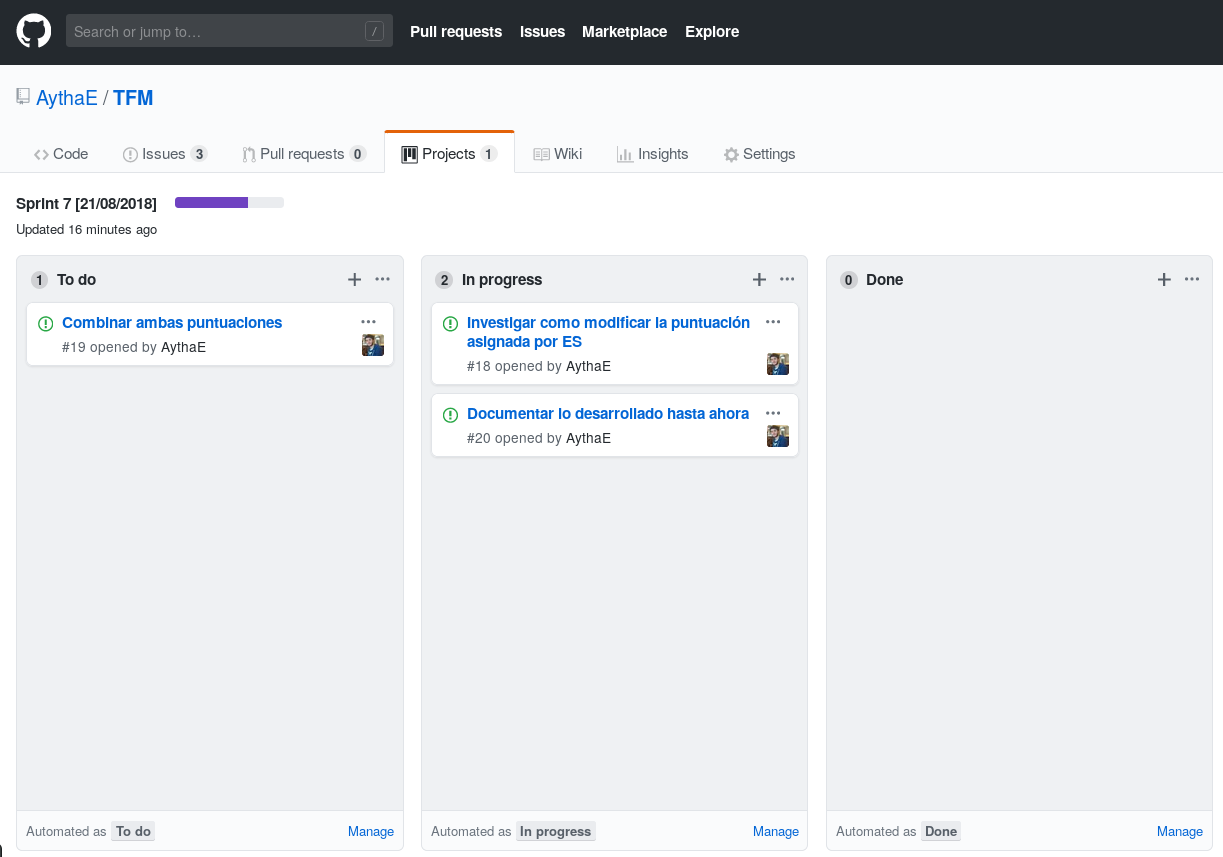
\includegraphics[width=\linewidth]{imagenes/ejemplo_tablero_sprint}
	\caption{Ejemplo de tablero de un \textit{sprint}}
	\label{fig:tableroSprint}
\end{figure}

Además de esto he utilizado un archivo \textit{Markdown} a modo de diario donde ir apuntando cosas interesantes según iban surgiendo, el estado actual de desarrollo o algunas tareas para completar próximamente, dicho fichero se llama \texttt{Diario.md}.

\section{Planificación temporal}

Desde la asignación del \acrshort{TFM}, en diciembre de 2017, me percaté que iba a ser realmente complicado alcanzar la primera convocatoria con la carga de trabajo que suponía el máster. Por lo que decidí tomarlo con calma y llegar a septiembre, pero tras todo finalizar el curso comencé la realización de mis prácticas, lo cual unido a lo extenuado que había acabado el año me impidió alcanzar otra vez el objetivo. 

En Octubre de 2017 comienzo a trabajar, lo cual suponen muchas horas menos al día y me llevo un tiempo adaptarme por lo que no fue hasta Febrero de 2018 cuando me lo empecé a tomar en serio. Teniendo en cuenta mi limitada disponibilidad horaria que apenas me permitía dedicarle 1-2 horas entre diario esbocé una planificación con el objeto de entregar el proyecto en Julio de 2018, dicha planificación inicial se recoge en la siguiente tabla.

\begin{table} [h!]
	\centering
	\begin{tabular}{l c c c}
		\hline
		\textbf{Tarea} & \textbf{Inicio} & \textbf{Fin} & \textbf{Duración}\\
		\hline\hline
		Investigación & 19/02/2018 & 23/04/2018 & 8 semanas \\
		\hline
		Obtención de datos & 23/04/2018 & 07/05/2018 & 2 semanas\\
		\hline
		Procesado de datos & 07/05/2018 & 21/05/2018 & 2 semanas\\
		\hline
		Búsqueda básica & 21/05/2018 & 04/06/2018 & 2 semanas\\
		\hline
		Búsqueda con bibliometría & 04/06/2018 & 02/07/2018 & 4 semanas\\
		\hline
		Refinamiento & 02/07/2018 & 09/07/2018 & 1 semana\\
		\hline
	
	\end{tabular}
	\caption{Planificación inicial de tareas}
\end{table}

Desgraciadamente las vacaciones que he tomado entre medias junto con algunos imprevistos no me permitieron llegar a tiempo aunque ya tenía el proyecto encaminado.
